\chapter{Przegląd istniejących rozwiązań w zakresie rozszerzonej rzeczywistości}
\label{cha:przegladIstniejacychRozwiazanWZakresieRozszerzonejRzeczywistosci}

W tym rozdziale zostało omówione kilka bibliotek implementujących narzędzia wykorzystywane w rozszerzonej rzeczywistości. W internecie można znaleźć dużo w tym także darmowych i open source bibliotek, które możemy wykorzystać do różnych programów na przykład gier, które wykorzystują rozszerzoną rzeczywistość.

%---------------------------------------------------------------------------

\section{Ogólne założenia systemów rozszerzonej rzeczywistości}
\label{sec:ogolneZalozeniaSystemowRozszerzonejRzeczywistosci}

Na początku warto wspomnieć o kilku ogólnych założeniach, które charakteryzują systemy rozszerzonej rzeczywistości. Poniżej w kilku punktach zostało opisane kilka cech takich systemów:
\begin{itemize}
	\item Obraz wirtualny bądź jego elementy nakładane są na obraz rzeczywisty uzyskany z kamery. Najczęściej punktem odniesienia są różnego rodzaju markery, jednakże mogą to być także różne charakterystyczne przedmioty otoczenia z pozyskanego obrazu rzeczywistego.
	\item Jednym z najtrudniejszych elementów w rozwijaniu aplikacji wykorzystujących rozszerzoną rzeczywistość jest dokładne obliczanie punktu widzenia użytkownika w czasie rzeczywistym, dzięki czemu wirtualne obrazy są dokładnie dostosowane do rzeczywistych obiektów.
	\item Obraz rzeczywisty ma zazwyczaj bardziej skomplikowane wymagania kalibracji kamery i rejestracji obrazu.
\end{itemize}

%---------------------------------------------------------------------------

\section{ARToolkit}
\label{sec:artoolkit}

Jest to jedna z najbardziej popularnych bibliotek open source wykorzystywanych w rozszerzonej rzeczywistości. Posiada także wiele rozszerzeń takich jak FLARToolkit i wiele podobnych. Kod źródłowy dla tego projektu jest zamieszczony na GitHub \cite{ARToolkit}, skompilowane SDK dla wszystkich platform (Mac OS X, PC, Linux, Android, iOS) wraz z wtyczką dla ARToolKit Unity3D, dostępne są na stronie głównej projektu \cite{ARToolkit}. Zaletami tej biblioteki są:
\begin{itemize}
	\item Solidne śledzenie markerów.
	\item Dobre wsparcie kalibracji kamery.
	\item Wieloplatformowe oraz posiada wpsarcie dla wielu języków programowania.
	\item Zoptymailizowane dla urządzeń mobilnych.
	\item Wsparcie dla unity3D oraz OpenSceneGraph.
\end{itemize}

ARToolKit wykorzystuje techniki wizualizacji komputerowej by obliczyć pozycję kamery i orientację względem kwadratowych kształtów lub płaskich powierzchni teksturowanych, pozwalając programiście nakładanie wirtualnych przedmiotów. ARToolKit obsługuje obecnie klasyczny kwadratowy znacznik, kod kreskowy 2D, wiele innych rodzajów markerów. Ponadto ARToolKit obsługuje dowolną kombinację powyższych razem. Szybkie, precyzyjne śledzenie dostarczone przez ARToolKit umożliwiło szybki rozwój tysiącu nowych i ciekawych aplikacji rozszerzonej rzeczywistości. ARToolkit obsługuje zarówno pliki wideo jaki obraz rzeczywisty bezpośrednio z kamerki.

Biblioteka opiera się na kwadratowych markerach składających się z białego tła oraz posiadających szeroką ciemną (zazwyczaj czarną) otoczkę wytyczającą granice markera. Konstrukcja ta czyni marker wyjątkowym, łatwym do rozpoznania. Są one rozpoznawane, wykrywane, a następnie używane do obliczania położenia w przestrzeni 3D. ARToolkit działa następująco:
\begin{itemize}
	\item Aparat rejestruje wideo w polu widzenia kamery i wysyła je do komputera.
	\item Oprogramowanie na komputerze przeszukuje każdą klatkę wideo dla dowolnych kształtów kwadratowych (markery kwadratowe).
	\item Jeśli kwadratowy marker zostanie znaleziony i treść obrazu osadzona przez wzór, jest dopasowana i zidentyfikowana to oprogramowanie wykorzystuje matematykę do obliczenia, w stosunku do aparatu, zarówno pozycję czarnego kwadratu jak i orientację wzoru.
	\item Gdy pozycja i orientacja kamery są znane, model grafiki komputerowej jest rysowany za pomocą położenia obliczonej pozycji i orientacji dopasowania.
	\item Model ten jest rysowany w planie przechwyconego wideo i są śledzone ruchy wideo w tle, a następnie model jest dołączany do tła.
	\item Wynikiem końcowym jest pokazany na wyświetlaczu obiekt w tle obrazu z kamery, więc widz widzi renderowany graficzny model nad strumieniem wideo świata rzeczywistego.
\end{itemize}
Rysunek 2.1 podsumowuje powyższe kroki.
\bigskip

\begin{figure}[ht!]
\centering
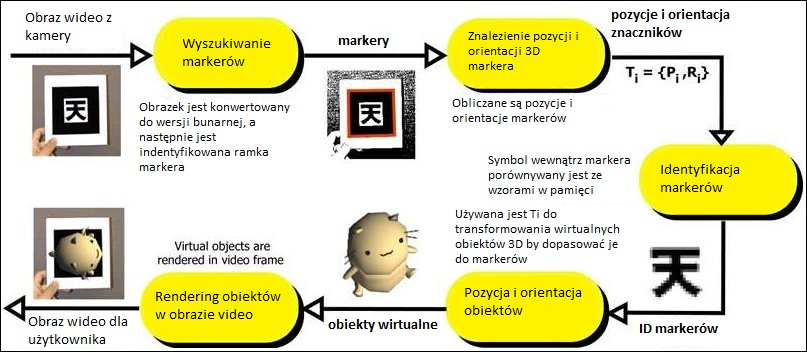
\includegraphics[width=150mm]{diagram.jpg}
\caption{Działanie ARToolkit krok po kroku \label{artoolkitsteps}}
\end{figure}

ARToolkit posiada jednak pewne ograniczenia. Obiekt wyświetlany jest tylko wtedy gdy marker jest w polu widzenia kamery. Jeżeli choć część markera zostanie czymś przysłonięta to wirtualny obiekt znika. Natomiast jeżeli granice markera będą poza polem widzenia kamery to obiekt zostanie obcięty. Istnieje również problem w zakresie śledzenia optycznego, ponieważ kiedy markery są przeniesione dalej od kamery to znaczniki zajmują mniej pikseli widzenia kamery i wynikiem jest posiadanie niewystarczającej ilości szczegółów by wyśledzić i zidentyfikować marker. Im większy fizycznie osadzony wzór markera tym dalej wzór markera można wykryć, a więc większa umiejętność wykrywania markera. Wreszcie, wyniki śledzenia są również zależne od warunków oświetleniowych. Zbyt mocne oświetlenie może tworzyć odbicia i odblaski (plamy) na paierowych markerach i tak sprawiają, że trudniej znaleźć kwadratowy marker. Cienie mogą być rzucone w poprzek papieru, rozbijając białe obszary na obrazie z kamery.

% %---------------------------------------------------------------------------

\section{ArUco}
\label{sec:aruco}



% %---------------------------------------------------------------------------

\section{Vuforia}
\label{sec:vuforia}


